\section{Interaction Region}
\label{section: interaction region}

The mean interaction region is described by two quantities, the beam line and the luminous region. The beamline is a vector quantity defined as being the axis along which the average proton-proton interactions occurs. This is calculated by plotting the $x$ and $y$ distribution of the primary vertex position as a function of $z$ and fitting them with a first order polynomial, see figures \ref{fig: pv_distributions mc mag down x_of_z} and \ref{fig: pv_distributions mc mag down y_of_z}. From these fits an equation of the beam line can be determined, the minimum distance between the track and the beam line gives the distance of closest approach (DOCA) between the track and beam line.

The luminous region describes the range of z values in which the proton-proton interactions occur. This is calculated by plotting the $z$ distribution of the primary vertices and fitting this distributions with a Gaussian giving its mean position and corresponding standard deviation from it, see figure \ref{fig: pv_distributions mc mag down z}.

%The mean interaction region is calculated from the position distribution of primary vertices in selected events. The x and y position of the primary vertex are plotted as a function of its z position and are fitted with a first order polynomial to give an equation for the beamline - the axis through which most proton-proton interactions occur on average. Examples of these fits are show in figure \ref{fig: pv_distributions mc mag down x_of_z} and \ref{fig: pv_distributions mc mag down y_of_z}.
%
%A distribution of the  z position of the primary vertex is also plotted. This is fitted with a Gaussian distribution giving the mean position in z where proton-proton collisions occur as well as the standard deviation from this region, see figure \ref{fig: pv_distributions mc mag down z}.

\begin{figure}[h]
	\centering
	\begin{subfigure}{0.49\textwidth}
		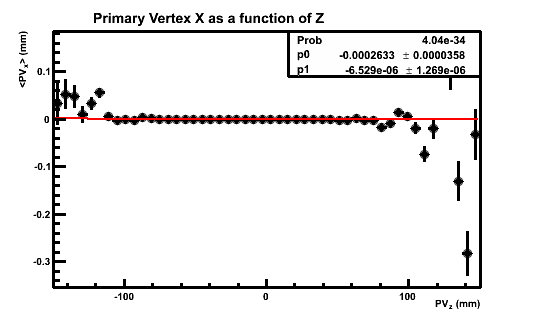
\includegraphics[width=\textwidth]{./Chapters/multiplicity/images/beamline_x_of_z.png}
		\caption{$\left<PV_x\right>$ as a function of $PV_z$}
		\label{fig: pv_distributions mc mag down x_of_z}
	\end{subfigure}
	\begin{subfigure}{0.49\textwidth}
		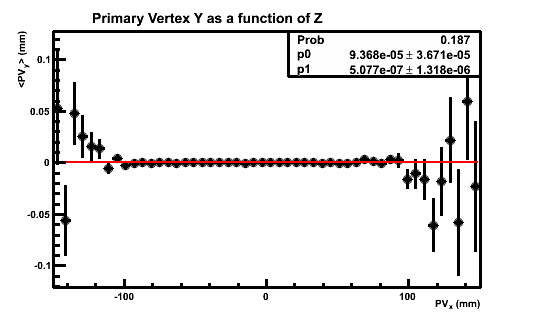
\includegraphics[width=\textwidth]{./Chapters/multiplicity/images/beamline_y_of_z.png}
		\caption{$\left<PV_y\right>$ as a function of $PV_z$}
		\label{fig: pv_distributions mc mag down y_of_z}
	\end{subfigure}
	\begin{subfigure}{0.49\textwidth}
		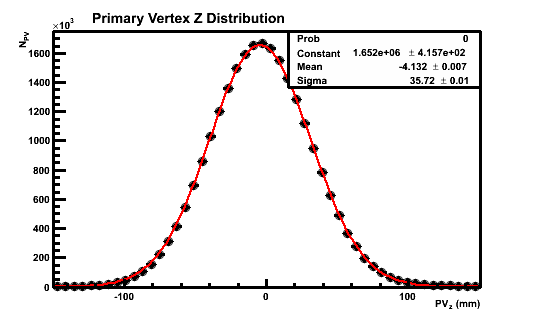
\includegraphics[width=\textwidth]{./Chapters/multiplicity/images/beamline_z.png}
		\caption{$PV_z$}
		\label{fig: pv_distributions mc mag down z}
	\end{subfigure}
	\caption{PV distributions of MC data in the magnet down configuration}
	\label{fig: pv distributions mc mag down}
\end{figure}